% DOCUMENT CLASS SETUP
\documentclass[12pt, a4paper]{article}

% DOCUMENT PACKAGES
\usepackage[a4paper, margin=1in]{geometry}
\usepackage{titling}
\usepackage{enumitem}
\usepackage{amsmath}
\usepackage{amssymb}
\usepackage{mathtools}
\usepackage{graphicx}
\usepackage{xcolor}
\usepackage{listings}
\usepackage{hyperref}

% FONT AND ENCODING SETUP
\usepackage[english]{babel}
\usepackage[utf8]{inputenc}
\usepackage[T1]{fontenc}
\usepackage{lmodern}
\usepackage{fontspec}

% PROFESSIONAL CODE BLOCK
\usepackage{tcolorbox}
\tcbuselibrary{minted, skins, breakable}

% DEFINE GITHUB DARK THEME COLORS %
\definecolor{ghback}{HTML}{0d1117}    % Dark background
\definecolor{ghtext}{HTML}{c9d1d9}    % Light gray text
\definecolor{ghborder}{HTML}{30363d}  % GitHub Border color

% PROFESSIONAL CODE BLOCK CONFIGURATION (MINTED VERSION) %
\renewcommand{\theFancyVerbLine}{\textcolor{white!60!gray}{\scriptsize\arabic{FancyVerbLine}}}
\newtcblisting{codeblock}[2][]{
    enhanced,
    breakable,
    colback=ghback,
    colframe=ghborder,
    coltitle=ghtext,
    fonttitle=\bfseries\small,
    arc=3mm,
    boxrule=0.5mm,
    % PADDING SETTINGS
    left=25pt,
    right=10pt,
    top=5pt,
    bottom=5pt,
    % MINTED SETTINGS
    listing engine=minted,
    listing only,
    minted language=python,
    minted options={
        linenos,
        numbersep=5pt,
        fontsize=\footnotesize,
        breaklines=true,
        autogobble,
        style=monokai,
    },
    title={#2},
    #1
}

% DEFINE DOCUMENT CUSTOM MARCOS %
\newcommand{\sol}{\par\noindent\underline{\textbf{Sol.}} }
\newcommand{\ans}{\par\noindent\underline{\textbf{Ans.}} }

% DOCUMENT TITLE SETUP %
\title {
	\textbf{2110573 PATTERN RECOGNITION} \\
    \vspace{1em}
	\Large{\textbf{Homework 4: Neural Networks}} \\
    \vspace{0.5em}
    \large{Computer Engineering, Chulalongkorn Univerity}
}
\author{Worralop Srichainont}
\date{\today}
\setlength{\droptitle}{15em}

% DOCUMENT CONTENTS
\begin{document}

    \maketitle
    \thispagestyle{empty}
    \clearpage

    \tableofcontents
    \thispagestyle{empty}
    \clearpage

    \pagenumbering{arabic}

    \section{The Basics}
        \subsection{Problem T1}
            Compute the forward and backward pass of the following computation. Note that this is simplified residual connection.
            \begin{align*}
                {x}_{1} &= \text{ReLU}({x}_{0} \ast {w}_{0} + {b}_{0}) \\
                {y}_{1} &= {x}_{1} \ast {w}_{1} + {b}_{1} \\
                z &= \text{ReLU}({y}_{1} + {x}_{0})
            \end{align*}

            Let $x_0 = 1.0$, $w_0 = 0.3$, $w_1 = -0.2$, $b_0 = 0.1$, $b_1 = -0.3$. Find the gradient of $z$ with respect to $w_0$, $w_1$, $b_0$, and $b_1$.

            \subsubsection{Forward Pass}
                \begin{table}[h]
                    \centering
                    \begin{tabular}{c|c|c}
                        $\begin{aligned}
                            {x}_{1} &= \text{ReLU}(({x}_{0} \cdot {w}_{0}) + {b}_{0}) \\
                            {x}_{1} &= \text{ReLU}((1.0 \cdot 0.3) + 0.1) \\
                            {x}_{1} &= \text{ReLU}(0.4) \\
                            {x}_{1} &= \text{max}(0.0, 0.4) \\
                            {x}_{1} &= 0.4
                        \end{aligned}$
                        &
                        $\begin{aligned}
                            {y}_{1} &= ({x}_{1} \cdot {w}_{1}) + {b}_{1} \\
                            {y}_{1} &= (0.4 \cdot -0.2) + (-0.3) \\
                            {y}_{1} &= -0.38
                        \end{aligned}$
                        &
                        $\begin{aligned}
                            z &= \text{ReLU}({y}_{1} + {x}_{0}) \\
                            z &= \text{ReLU}(-0.38 + 1.0) \\
                            z &= \text{ReLU}(0.62) \\
                            z &= \text{max}(0.00, 0.62) \\
                            z &= 0.62
                        \end{aligned}$
                        \\
                    \end{tabular}
                \end{table}

            \subsubsection{Backward Pass}
                The problem required to calculate the gradient of $z$ with respect to ${w}_{0}$, ${w}_{1}$, ${b}_{0}$ and ${b}_{1}$.
                \begin{align*}
                    \frac{\partial z}{\partial {w}_{0}} &= \frac{\partial z}{\partial {y}_{1}} \cdot \frac{\partial {y}_{1}}{\partial {x}_{1}} \cdot \frac{\partial {x}_{1}}{\partial {w}_{0}} \\[1em]
                    \frac{\partial z}{\partial {w}_{1}} &= \frac{\partial z}{\partial {y}_{1}} \cdot \frac{\partial {y}_{1}}{\partial {w}_{1}} \\[1em]
                    \frac{\partial z}{\partial {b}_{0}} &= \frac{\partial z}{\partial {y}_{1}} \cdot \frac{\partial {y}_{1}}{\partial {x}_{1}} \cdot \frac{\partial {x}_{1}}{\partial {b}_{0}} \\[1em]
                    \frac{\partial z}{\partial {b}_{1}} &= \frac{\partial z}{\partial {y}_{1}} \cdot \frac{\partial {y}_{1}}{\partial {b}_{1}}
                \end{align*}

                \begin{align*}
                    \intertext{First, calculate $\frac{\partial z}{\partial {y}_{1}}$ and given $u = {y}_{1} + {x}_{0} = 0.62$}
                    \frac{\partial z}{\partial {y}_{1}} &= \frac{\partial z}{\partial u} \cdot \frac{\partial u}{\partial {y}_{1}} \\[1em]
                    \frac{\partial z}{\partial {y}_{1}} &= \frac{\partial}{\partial u}(\text{ReLU}(u)) \cdot \frac{\partial}{\partial {y}_{1}}({y}_{1} + {x}_{0}) \\[1em]
                    \intertext{As we can see that $u > 0$ which means ReLU(u) = u}
                    \frac{\partial z}{\partial {y}_{1}} &= \frac{\partial}{\partial u}(u) \cdot 1 \\[1em]
                    \frac{\partial z}{\partial {y}_{1}} &= 1.0 \tag{1}
                \end{align*}

                \begin{align*}
                    \intertext{Next, calculate $\frac{\partial {y}_{1}}{\partial {x}_{1}}$}
                    \frac{\partial {y}_{1}}{\partial {x}_{1}} &= \frac{\partial}{\partial {x}_{1}} \left( ({x}_{1} \cdot {w}_{1}) + {b}_{1} \right) \\[1em]
                    \frac{\partial {y}_{1}}{\partial {x}_{1}} &= {w}_{1} \\[1em]
                    \frac{\partial {y}_{1}}{\partial {x}_{1}} &= -0.2 \tag{2}
                \end{align*}

                \begin{align*}
                    \intertext{Next, calculate $\frac{\partial {y}_{1}}{\partial {w}_{1}}$}
                    \frac{\partial {y}_{1}}{\partial {w}_{1}} &= \frac{\partial}{\partial {w}_{1}} \left( ({x}_{1} \cdot {w}_{1}) + {b}_{1} \right) \\[1em]
                    \frac{\partial {y}_{1}}{\partial {w}_{1}} &= {x}_{1} \\[1em]
                    \frac{\partial {y}_{1}}{\partial {w}_{1}} &= 0.4 \tag{3}
                \end{align*}

                \begin{align*}
                    \intertext{Next, calculate $\frac{\partial {y}_{1}}{\partial {b}_{1}}$}
                    \frac{\partial {y}_{1}}{\partial {b}_{1}} &= \frac{\partial}{\partial {b}_{1}} \left( ({x}_{1} \cdot {w}_{1}) + {b}_{1} \right) \\[1em]
                    \frac{\partial {y}_{1}}{\partial {b}_{1}} &= 1.0 \tag{4}
                \end{align*}

                \begin{align*}
                    \intertext{Next, calculate $\frac{\partial {x}_{1}}{\partial {w}_{0}}$ and given $u = ({x}_{0} \cdot {w}_{0}) + {b}_{0} = 0.4$}
                    \frac{\partial {x}_{1}}{\partial {w}_{0}} &= \frac{\partial {x}_{1}}{\partial u} \cdot \frac{\partial u}{\partial {w}_{0}} \\[1em]
                    \frac{\partial {x}_{1}}{\partial {w}_{0}} &= \frac{\partial}{\partial u}(\text{ReLU}(u)) \cdot \frac{\partial}{\partial {w}_{0}}(({x}_{0} \cdot {w}_{0}) + {b}_{0}) \\[1em]
                    \intertext{As we can see that $u > 0$ which means ReLU(u) = u}
                    \frac{\partial z}{\partial {y}_{1}} &= \frac{\partial}{\partial u}(u) \cdot {x}_{0} \\[1em]
                    \frac{\partial z}{\partial {y}_{1}} &= 1.0 \tag{5}
                \end{align*}

                \begin{align*}
                    \intertext{Next, calculate $\frac{\partial {x}_{1}}{\partial {b}_{0}}$ and given $u = ({x}_{0} \cdot {w}_{0}) + {b}_{0} = 0.4$}
                    \frac{\partial {x}_{1}}{\partial {b}_{0}} &= \frac{\partial {x}_{1}}{\partial u} \cdot \frac{\partial u}{\partial {b}_{0}} \\[1em]
                    \frac{\partial {x}_{1}}{\partial {b}_{0}} &= \frac{\partial}{\partial u}(\text{ReLU}(u)) \cdot \frac{\partial}{\partial {b}_{0}}(({x}_{0} \cdot {w}_{0}) + {b}_{0}) \\[1em]
                    \intertext{As we can see that $u > 0$ which means ReLU(u) = u}
                    \frac{\partial z}{\partial {y}_{1}} &= \frac{\partial}{\partial u}(u) \cdot 1 \\[1em]
                    \frac{\partial z}{\partial {y}_{1}} &= 1.0 \tag{6}
                \end{align*}

                \noindent Finally, calculate the gradient of $z$ with respect to ${w}_{0}$, ${w}_{1}$, ${b}_{0}$ and ${b}_{1}$
                \begin{table}[h]
                    \centering
                    \begin{tabular}{c|c}
                        $\begin{aligned}
                            \frac{\partial z}{\partial {w}_{0}} &= \frac{\partial z}{\partial {y}_{1}} \cdot \frac{\partial {y}_{1}}{\partial {x}_{1}} \cdot \frac{\partial {x}_{1}}{\partial {w}_{0}} \\[1em]
                            \frac{\partial z}{\partial {w}_{0}} &= 1.0 \cdot (-0.2) \cdot 1.0 \\[1em]
                            \frac{\partial z}{\partial {w}_{0}} &= -0.2 \\[1em]
                        \end{aligned}$
                        &
                        $\begin{aligned}
                            \frac{\partial z}{\partial {w}_{1}} &= \frac{\partial z}{\partial {y}_{1}} \cdot \frac{\partial {y}_{1}}{\partial {w}_{1}} \\[1em]
                            \frac{\partial z}{\partial {w}_{1}} &= 1.0 \cdot 0.4 \\[1em]
                            \frac{\partial z}{\partial {w}_{1}} &= 0.4 \\[1em]
                        \end{aligned}$
                        \\
                        \hline
                        $\begin{aligned}
                            \\
                            \frac{\partial z}{\partial {b}_{0}} &= \frac{\partial z}{\partial {y}_{1}} \cdot \frac{\partial {y}_{1}}{\partial {x}_{1}} \cdot \frac{\partial {x}_{1}}{\partial {b}_{0}} \\[1em]
                            \frac{\partial z}{\partial {b}_{0}} &= 1.0 \cdot (-0.2) \cdot 1.0 \\[1em]
                            \frac{\partial z}{\partial {b}_{0}} &= -0.2 \\[1em]
                        \end{aligned}$
                        &
                        $\begin{aligned}
                            \\
                            \frac{\partial z}{\partial {b}_{1}} &= \frac{\partial z}{\partial {y}_{1}} \cdot \frac{\partial {y}_{1}}{\partial {b}_{1}} \\[1em]
                            \frac{\partial z}{\partial {b}_{1}} &= 1.0 \cdot 1.0 \\[1em]
                            \frac{\partial z}{\partial {b}_{1}} &= 1.0 \\[1em]
                        \end{aligned}$
                        \\
                    \end{tabular}
                \end{table}

    \pagebreak

        \subsection{Problem T2}
            Given the following network architecture specifications, determine the size of the output A, B, and C.

            \begin{table}[h]
                \centering
                \begin{tabular}{|c|c|}
                    \hline
                    Layer & Data Size \\
                    \hline
                    Input Layer & (32, 30) \\
                    Layer A & (32, 1,024) \\
                    Layer B & (32, 512) \\
                    Layer C & (32, 1) \\
                    \hline
                \end{tabular}
                \caption{Data Size in Layer}
            \end{table}

        \subsection{Problem T3}
            What is the total number of learnable parameters in this network?
            \begin{table}[h]
                \centering
                \begin{tabular}{|c|c|c|c|c|}
                    \hline
                    Layer & Inputs & Neurons & Bias & Parameters \\
                    \hline
                    Layer A & 30 & 1,024 & 1,024 & $(30 \times 1,024) + 1,024 = 31,744$ \\
                    Layer B & 1,024 & 512 & 512 & $(1,024 \times 512) + 512 = 524,800$ \\
                    Layer C & 512 & 1 & 1 & $(512 \times 1) + 1 = 513$ \\
                    \hline
                \end{tabular}
                \caption{Parameters in Layer}
            \end{table}
            
            So this neural network would have 31,744 + 524,800 + 513 = 557,057 parameters in total.

            \ans 557,057 parameters
    
    \pagebreak

    \section{Deep Learning from (almost) scratch}

        In this section we will code simple a neural network model from scratch (numpy). However, before we go into coding let's start with some loose ends, namely the gradient of the softmax layer.

        Recall in class we define the softmax layer as:
        \begin{equation}
            P(y=j) = \frac{\exp(h_j)}{\Sigma_k \exp(h_k)}
        \end{equation}
        where $h_j$ is the output of the previous layer for class index $j$

        The cross entropy loss is defined as:
        \begin{equation}
            L = -\Sigma_j \left( y_j \cdot \log P(y=j) \right)
        \end{equation}
        where $y_j$ is 1 if $y$ is class $j$, and 0 otherwise.

        \subsection{Problem T4}
            Prove that the derivative of the loss with respect to $h_i$ is $P(y=i) - y_i$.
            In other words, find $\frac{\partial L}{\partial h_i}$ for $i \in \{0, \dots, N-1\}$ where $N$ is the number of classes.

            \noindent Hint: first find $\frac{\partial P(y=j)}{\partial h_i}$ for the case where $j = i$, and the case where $j \neq i$.
            Then, use the results with chain rule to find the derivative of the loss.

            \subsubsection{Prove I}
                \noindent Calculate $\frac{\partial P(y=j)}{\partial h_i}$ for the case where $j = i$
                \begin{align*}
                    \frac{\partial P(y=i)}{\partial h_i} &= \frac{\partial}{\partial h_i} \left( \frac{\exp(h_i)}{\Sigma_k \exp(h_k)} \right) \\[1em]
                    \frac{\partial P(y=i)}{\partial h_i} &= \frac{
                        \left( \Sigma_k \exp(h_k)  \right) \left( \frac{\partial}{\partial h_i} \left( \exp(h_i) \right) \right)
                        - \left( \exp(h_i)  \right) \left( \frac{\partial}{\partial h_i} \left( \Sigma_k \exp(h_k) \right) \right)
                    }
                    {{\left( \Sigma_k \exp(h_k) \right)}^{2}} \\[1em]
                    \intertext{For a term which $k \neq i$ in $\Sigma_k \exp(h_k)$ has its partial derivative equal to 0}
                    \intertext{
                        In other words, $\frac{\partial}{\partial h_i} \left( \Sigma_k \exp(h_k) \right)
                        = 0 + \dots + \frac{\partial}{\partial h_i} \exp(h_i) + \dots + 0
                        = \exp(h_i)$
                    }
                    \frac{\partial P(y=i)}{\partial h_i} &= \frac{
                        \left( \Sigma_k \exp(h_k)  \right) \left( \exp(h_i) \right)
                        - {\left( \exp(h_i)  \right)}^{2}
                    }
                    {{\left( \Sigma_k \exp(h_k) \right)}^{2}} \\[1em]
                    \frac{\partial P(y=i)}{\partial h_i} &= \frac{\exp(h_i)}{\Sigma_k \exp(h_k)} \left(
                        \frac{\Sigma_k \exp(h_k) - \exp(h_i)}{\Sigma_k \exp(h_k)}
                    \right)\\[1em]
                    \frac{\partial P(y=i)}{\partial h_i} &= \frac{\exp(h_i)}{\Sigma_k \exp(h_k)} \left(
                        1 - \frac{\exp(h_i)}{\Sigma_k \exp(h_k)}
                    \right) \\[1em]
                    \frac{\partial P(y=i)}{\partial h_i} &= P(y=i) \cdot (1 - P(y=i))
                \end{align*}

    \pagebreak

                \noindent Calculate $\frac{\partial P(y=j)}{\partial h_i}$ for the case where $j \neq i$
                \begin{align*}
                    \frac{\partial P(y=j)}{\partial h_i} &= \frac{\partial}{\partial h_i} \left( \frac{\exp(h_j)}{\Sigma_k \exp(h_k)} \right) \\[1em]
                    \frac{\partial P(y=j)}{\partial h_i} &= \frac{
                        \left( \Sigma_k \exp(h_k)  \right) \left( \frac{\partial}{\partial h_i} \left( \exp(h_j) \right) \right)
                        - \left( \exp(h_j) \right) \left( \frac{\partial}{\partial h_i} \left( \Sigma_k \exp(h_k) \right) \right)
                    }
                    {{\left( \Sigma_k \exp(h_k) \right)}^{2}} \\[1em]
                    \intertext{
                        For a term $\frac{\partial}{\partial h_i} \left( \exp(h_j) \right)$ is equal to 0 because $j \neq i$
                    }
                    \frac{\partial P(y=j)}{\partial h_i} &= - \frac{
                        \left( \exp(h_j) \right)
                        \left( \frac{\partial}{\partial h_i} \left( \Sigma_k \exp(h_k) \right) \right)
                    }
                    {{\left( \Sigma_k \exp(h_k) \right)}^{2}} \\[1em]
                    \intertext{For a term which $k \neq i$ in $\Sigma_k \exp(h_k)$ has its partial derivative equal to 0}
                    \intertext{
                        In other words, $\frac{\partial}{\partial h_i} \left( \Sigma_k \exp(h_k) \right)
                        = 0 + \dots + \frac{\partial}{\partial h_i} \exp(h_i) + \dots + 0
                        = \exp(h_i)$
                    }
                    \frac{\partial P(y=j)}{\partial h_i} &= - \frac{
                        \left( \exp(h_j) \right) \left( \exp(h_i) \right)
                    }
                    {{\left( \Sigma_k \exp(h_k) \right)}^{2}} \\[1em]
                    \frac{\partial P(y=j)}{\partial h_i} &= - \frac{\exp(h_j)}{\Sigma_k \exp(h_k)}
                    \cdot \frac{\exp(h_i)}{\Sigma_k \exp(h_k)} \\[1em]
                    \frac{\partial P(y=j)}{\partial h_i} &= -P(y=j) \cdot P(y=i)
                \end{align*}

                Thus, we can prove that
                \begin{align*}
                    \frac{\partial P(y=j)}{\partial h_i} =
                    \begin{dcases}
                        P(y=i) \cdot (1 - P(y=i)) & \text{if } j = i \\
                        -P(y=j) \cdot P(y=i) & \text{if } j \neq i
                    \end{dcases}
                \end{align*}

    \pagebreak

            \subsubsection{Prove II}
                After finishing calculate $\frac{\partial P(y=j)}{\partial h_i}$, we are going to calculate $\frac{\partial L}{\partial h_i}$ next.
                \begin{align*}
                    \frac{\partial L}{\partial h_i} &= \frac{\partial}{\partial h_i} \left( -\sum_j \left( y_j \cdot \log P(y=j) \right) \right) \\[1em]
                    \frac{\partial L}{\partial h_i} &= -\sum_j \left( \frac{\partial}{\partial h_i} \left( y_j \cdot \log P(y=j) \right) \right) \\[1em]
                    \frac{\partial L}{\partial h_i} &= -\sum_j \left(
                        \frac{\partial}{\partial P(y=j)} \left( y_j \cdot \log P(y=j) \right)
                        \cdot \frac{\partial P(y=j)}{\partial h_i}
                    \right) \\[1em]
                    \frac{\partial L}{\partial h_i} &= -\sum_j \left(
                        \left( y_j \cdot \frac{1}{P(y=j)} \right)
                        \cdot \frac{\partial P(y=j)}{\partial h_i}
                    \right) \\[1em]
                    \intertext{We need to separate the summation into 2 parts which are the summation of all terms where $j \neq i$ and a term where $j = i$.}
                    \frac{\partial L}{\partial h_i} &= -\sum_{j \neq i} \left(
                        \frac{y_j}{P(y=j)} \cdot \frac{\partial P(y=j)}{\partial h_i}
                    \right)
                    - \left(
                        \frac{y_i}{P(y=i)} \cdot \frac{\partial P(y=i)}{\partial h_i}
                    \right) \\[1em]
                    \intertext{Substitute $\frac{\partial P(y=j)}{\partial h_i}$ from the previous section.}
                    \frac{\partial L}{\partial h_i} &= -\sum_{j \neq i} \left(
                        \frac{y_j (-P(y=j) \cdot P(y=i))}{P(y=j)}
                    \right)
                    - \frac{y_i (P(y=i) \cdot (1 - P(y=i)))}{P(y=i)} \\[1em]
                    \frac{\partial L}{\partial h_i} &= \sum_{j \neq i} \left( y_j \cdot P(y=i) \right) - y_i(1 - P(y=i)) \\[1em]
                    \frac{\partial L}{\partial h_i} &= \left( P(y=i) \cdot \sum_{j \neq i} (y_j) \right) - y_i + (P(y=i) \cdot y_i) \\[1em]
                    \frac{\partial L}{\partial h_i} &= P(y=i) \cdot \left( \sum_{j \neq i} (y_j) + y_i \right) - y_i \\[1em]
                    \frac{\partial L}{\partial h_i} &= \left( P(y=i) \cdot \sum_{j} (y_j) \right) - y_i \\[1em]
                    \intertext{Since $y_i = 1$ if $i = j$ and $y_i = 0$ if $i \neq j$, it means $\Sigma_k (y_k) = 1$}
                    \frac{\partial L}{\partial h_i} &= P(y=i) - y_i
                \end{align*}

    \pagebreak

    \section{Two-Layer Neural Networks}
        In this part of the homework, we will work on building a simple Neural Network to classify digits using MNIST dataset.
        There are many powerful neural network frameworks nowadays that are relatively straightforward to use.
        However, we believe that in order to understand the theory behind neural networks, and to have the right intuitions in order to build, use, and debug more complex architectures, one must first start from the basics.

        Your task is to complete the missing codes needed for training and testing of a simple fully-connected neural network.

        \textbf{You can access the Colab Notebook using this link: \\ \text{\url{https://colab.research.google.com/drive/1u_oy5Fmw17iyrO2CckBoZ4yWC4GcQiGA}}}

        \subsection{Problem T5}
            \subsubsection{Implementation}
                Open the file \texttt{cattern/neural\_net.py} and look at the method \texttt{TwoLayerNet.loss}.
                This function takes the data and weights and computes the class scores, the loss, and the gradients on the parameters.

                For the problem T5, please perform the forward pass, computing the class scores for the input.
                Store the result in the scores variable, which should be an array of shape (N, C). Note that this does not include the softmax

                To calculate the class score for the next layer, it is just the matrix multiplication.
                \begin{align*}
                    \begin{bmatrix}
                        {{x}_{0}}^{(1)} \\
                        {{x}_{1}}^{(1)} \\
                        \vdots \\
                        {{x}_{n - 1}}^{(1)} \\
                        {{x}_{n}}^{(1)} \\
                    \end{bmatrix}
                    &=
                    \text{ReLU}
                    \left(
                    \begin{bmatrix}
                        {{w}_{0, 0}}^{(0)} & {{w}_{0, 1}}^{(0)} & \dots & {{w}_{0, k}}^{(0)} \\
                        {{w}_{1, 0}}^{(0)} & {{w}_{1, 1}}^{(0)} & \dots & {{w}_{1, k}}^{(0)} \\
                        \vdots & \vdots & \ddots & \vdots\\
                        {{w}_{n - 1, 0}}^{(0)} & {{w}_{n - 1, 1}}^{(0)} & \dots & {{w}_{n - 1, k}}^{(0)} \\
                        {{w}_{n, 0}}^{(0)} & {{w}_{n, 1}}^{(0)} & \dots & {{w}_{n, k}}^{(0)} \\
                    \end{bmatrix}
                    \cdot
                    \begin{bmatrix}
                        {{x}_{0}}^{(0)} \\
                        {{x}_{1}}^{(0)} \\
                        \vdots \\
                        {{x}_{n - 1}}^{(0)} \\
                        {{x}_{n}}^{(0)} \\
                    \end{bmatrix}
                    +
                    \begin{bmatrix}
                        {{b}_{0}}^{(0)} \\
                        {{b}_{1}}^{(0)} \\
                        \vdots \\
                        {{b}_{n - 1}}^{(0)} \\
                        {{b}_{n}}^{(0)} \\
                    \end{bmatrix}
                    \right)
                \end{align*}
                \begin{codeblock}{Problem T5}
                    class TwoLayerNet(object):
                        def loss(self, X, y=None, reg=0.0):
                            # Unpack variables from the params dictionary
                            W1, b1 = self.params["W1"], self.params["b1"]
                            W2, b2 = self.params["W2"], self.params["b2"]
                            N, D = X.shape

                            # Compute the forward pass
                            scores = None

                            # ==================== BEGIN OF T5 ====================
                            # Calculate class score in the hidden layer.
                            z1 = X.dot(W1) + b1

                            # Apply ReLU activation function
                            a1 = np.maximum(0, z1)

                            # Calculate class score in the output layer.
                            scores = a1.dot(W2) + b2
                            # ===================== END OF T5 =====================
                \end{codeblock}

    \pagebreak

            \subsubsection{Testing}
                In this part, we are generating the test data using the following function:
                \begin{codeblock}{Generate Test Data}
                    def init_toy_data():
                        np.random.seed(1)
                        X = 10 * np.random.randn(num_inputs, input_size)
                        y = np.array([0, 1, 2, 2, 1])
                        return X, y
                \end{codeblock}

                Next, we are going to calculate the class score from the implementation and found out that the difference from the correct class score is $3.68 \times {10}^{-8}$ which is acceptable because it is less than ${10}^{-7}$.

    \pagebreak

        \subsection{Problem T6}
            For the problem T6, please implement the second part that computes the data and regularization loss.

            To convert score to probability, use softmax function which has the formula below:
            \begin{equation}
                P(y=i) = \frac{\exp(h_i)}{\Sigma_k \exp(h_k)}
            \end{equation}

            Then, calculate data loss using the following formula:
            \begin{equation}
                \text{Data Loss} = - \log({\text{Probability}}_{\text{correct}})
            \end{equation}

            Next, calculate L2 regularization loss by using the following formula:
            \begin{equation}
                \text{L2 Regularization Loss} = \frac{1}{2} \cdot \lambda \cdot \sum ({w}^{2})
            \end{equation}

            Finally, calculate the total loss by the following equation:
            \begin{equation}
                \text{Total Loss} = \text{Data Loss} + \text{L2 Regularization Loss}
            \end{equation}

            \begin{codeblock}{Problem T6}
                class TwoLayerNet(object):
                    def loss(self, X, y=None, reg=0.0):
                        # ALL CODE BEFORE T6...

                        # ==================== BEGIN OF T6 ====================
                        # Subtract by max score to prevent overflow, then apply softmax function.
                        shift_scores = scores - np.max(scores, axis=1, keepdims=True)
                        exp_scores = np.exp(shift_scores)
                        probs = exp_scores / np.sum(exp_scores, axis=1, keepdims=True)

                        # Calculate log probability of only the correct class.
                        correct_logprobs = -np.log(probs[range(N), y])
                        data_loss = np.sum(correct_logprobs) / N

                        # Calculate L2 regularization loss
                        reg_loss = 0.5 * reg * np.sum(W1 * W1) + 0.5 * reg * np.sum(W2 * W2)

                        # Calculate the total loss
                        loss = data_loss + reg_loss
                        # ===================== END OF T6 =====================
            \end{codeblock}

            After that, perform a test by using the same test data from the previous problem to calculate the total loss and compare with the correct loss. The difference from the correct loss is $1.80 \times {10}^{-13}$ which is acceptable because it is less than ${10}^{-12}$.

    \pagebreak

        \subsection{Problem T7}
            For the problem T7, please compute the backward pass, computing derivatives of the weights and biases.
            Store the results in the \texttt{grads} dictionary.

            \begin{codeblock}{Problem T7}
                class TwoLayerNet(object):
                    def loss(self, X, y=None, reg=0.0):
                        # ALL CODE BEFORE T7...

                        # ==================== BEGIN OF T7 ====================
                        # Backward pass: compute gradients
                        grads = {}

                        # Calculate the gradient with respect to the loss scores
                        dscores = probs
                        dscores[range(N), y] -= 1
                        dscores /= N

                        # Calculate the gradient with respect to W2 and b2
                        grads["W2"] = a1.T.dot(dscores) + reg * W2
                        grads["b2"] = np.sum(dscores, axis=0)

                        # Pass gradient back to hidden layer
                        da1 = dscores.dot(W2.T)

                        # Backpropagation through ReLU
                        dz1 = da1
                        dz1[a1 <= 0] = 0

                        # Calculate the gradient with respect to W1 and b1
                        grads["W1"] = X.T.dot(dz1) + reg * W1
                        grads["b1"] = np.sum(dz1, axis=0)

                        return loss, grads
                        # ===================== END OF T7 =====================
            \end{codeblock}

            After that, perform a test by calculating the gradient, then comparing with the analytic gradient to calculate the relative error.
            \begin{itemize}
                \item Max relative error of $W_2$ is $3.44 \times {10}^{-9}$
                \item Max relative error of $W_2$ is $3.87 \times {10}^{-11}$
                \item Max relative error of $W_2$ is $3.56 \times {10}^{-9}$
                \item Max relative error of $W_2$ is $1.56 \times {10}^{-9}$
            \end{itemize}
            These are acceptable because they are all less than ${10}^{-8}$.

    \pagebreak

        \subsection{Problem T8}
            For the problem T8, please create a random mini-batch of training data and labels, storing them in \texttt{X\_batch} and \texttt{y\_batch} respectively.

            \begin{codeblock}{Problem T8}
                class TwoLayerNet(object):
                    def train(
                        self, X, y, X_val, y_val,
                        learning_rate=1e-3,
                        learning_rate_decay=0.95,
                        reg=5e-6,
                        num_iters=100,
                        batch_size=200,
                        verbose=False,
                    ):
                        num_train = X.shape[0]
                        iterations_per_epoch = max(num_train / batch_size, 1)

                        # Use SGD to optimize the parameters in self.model
                        loss_history = []
                        train_acc_history = []
                        val_acc_history = []

                        for it in range(num_iters):
                            X_batch = None
                            y_batch = None

                            # ==================== BEGIN OF T8 ====================
                            # Generate random indices
                            indices = np.random.choice(num_train, batch_size)

                            # Select the specific rows for images and labels
                            X_batch = X[indices]
                            y_batch = y[indices]
                            # ===================== END OF T8 =====================
            \end{codeblock}

    \pagebreak

        \subsection{Problem T9}
            For the problem T9, please use the gradients in the grads dictionary to update the parameters of the network using stochastic gradient descent.

            \begin{codeblock}{Problem T9}
                class TwoLayerNet(object):
                    def train(
                        self, X, y, X_val, y_val,
                        learning_rate=1e-3,
                        learning_rate_decay=0.95,
                        reg=5e-6,
                        num_iters=100,
                        batch_size=200,
                        verbose=False,
                    ):
                        # ALL OUTER LOOP CODE BEFORE T9...

                        for it in range(num_iters):
                            # ALL INNER LOOP CODE BEFORE T9...

                            # ==================== BEGIN OF T9 ====================
                            # Compute loss and gradients using the current minibatch
                            loss, grads = self.loss(X_batch, y=y_batch, reg=reg)
                            loss_history.append(loss)

                            # Update all parameters using the gradients and learning rate
                            self.params["W1"] -= learning_rate * grads["W1"]
                            self.params["b1"] -= learning_rate * grads["b1"]
                            self.params["W2"] -= learning_rate * grads["W2"]
                            self.params["b2"] -= learning_rate * grads["b2"]
                            # ===================== END OF T9 =====================
            \end{codeblock}

    \pagebreak

        \subsection{Problem T10}
            For the problem T10, please calculate decay learning rate (exponentially) after each epoch.
            \subsubsection{Implementation}
                \begin{codeblock}{Problem T10}
                    class TwoLayerNet(object):
                        def train(
                            self, X, y, X_val, y_val,
                            learning_rate=1e-3,
                            learning_rate_decay=0.95,
                            reg=5e-6,
                            num_iters=100,
                            batch_size=200,
                            verbose=False,
                        ):
                            # ALL OUTER LOOP CODE BEFORE T10...

                            for it in range(num_iters):
                                # ALL INNER LOOP CODE BEFORE T10...

                                if verbose and it % 100 == 0:
                                    print("iteration %d / %d: loss %f" % (it, num_iters, loss))

                                # Every epoch, check train and val accuracy and decay learning rate.
                                if it % iterations_per_epoch == 0:
                                    # Check accuracy
                                    train_acc = (self.predict(X_batch) == y_batch).mean()
                                    val_acc = (self.predict(X_val) == y_val).mean()
                                    train_acc_history.append(train_acc)
                                    val_acc_history.append(val_acc)

                                    # ==================== BEGIN OF T10 ====================
                                    learning_rate *= learning_rate_decay
                                    # ===================== END OF T10 =====================
            
                            return {
                                "loss_history": loss_history,
                                "train_acc_history": train_acc_history,
                                "val_acc_history": val_acc_history,
                            }
                \end{codeblock}

    \pagebreak

            \subsubsection{Evaluation}
                After implementation in problem T8 - T10, we plot the training loss from the test data from the problem T5 during the model training process as shown below:
                \begin{figure}[h]
                    \centering
                    
\includegraphics[width=0.8\textwidth]{image_01}
                    \caption{Model Training Loss}
                \end{figure}

                The training loss of the model at the final epoch is 0.017 which is acceptable because the model achieve a training loss less than 0.05.

    \pagebreak

        \subsection{Problem T11}
            \subsubsection{Implementation}
                For the problem T11, please implement \texttt{predict()} function.

                \begin{codeblock}{Problem T11}
                    class TwoLayerNet(object):
                        def predict(self, X):
                            y_pred = None

                            # ==================== BEGIN OF T11 ====================
                            # Forward pass the test set.
                            h1 = np.maximum(0, X.dot(self.params["W1"]) + self.params["b1"])
                            scores = h1.dot(self.params["W2"]) + self.params["b2"]

                            # Choose class with the highest score
                            y_pred = np.argmax(scores, axis=1)
                            # ===================== END OF T11 =====================

                            return y_pred
                \end{codeblock}
            
            \subsubsection{Load MNIST Dataset}
                Since we are finish with the neural network implementation, we are going to apply MNIST dataset to the model.

                First, load the dataset using the following code:

                \begin{codeblock}{Load MNIST Dataset}
                    from mnist_data import load_mnist

                        def get_mnist_data(num_training=55000, num_validation=5000, num_test=10000):
                            # Load the raw MNIST data
                            X_train, y_train, X_val, y_val, X_test, y_test = load_mnist.read_data_sets(
                                "mnist_data"
                            )

                            # Normalize the data: subtract the mean image
                            mean_image = np.mean(X_train, axis=0)
                            X_train = X_train - mean_image
                            X_val = X_val - mean_image
                            X_test = X_test - mean_image

                            # Reshape data to rows
                            X_train = X_train.reshape(num_training, -1)
                            X_val = X_val.reshape(num_validation, -1)
                            X_test = X_test.reshape(num_test, -1)

                            return X_train, y_train, X_val, y_val, X_test, y_test

                        X_train, y_train, X_val, y_val, X_test, y_test = get_mnist_data()
                \end{codeblock}

    \pagebreak

                The shape of the dataset are:
                \begin{table}[h]
                    \centering
                    \begin{tabular}{|c|c|}
                        \hline
                        Dataset & Data Shape \\
                        \hline \hline
                        Train dataset & (55000, 784) \\
                        Train labels & 55000 \\
                        \hline
                        Validation dataset & (5000, 784) \\
                        Validation labels & 5000 \\
                        \hline
                        Test dataset & (10000, 784) \\
                        Test labels & 10000 \\
                        \hline
                    \end{tabular}
                    \caption{Dataset Shape}
                \end{table}

            \begin{figure}[h]
                \centering
                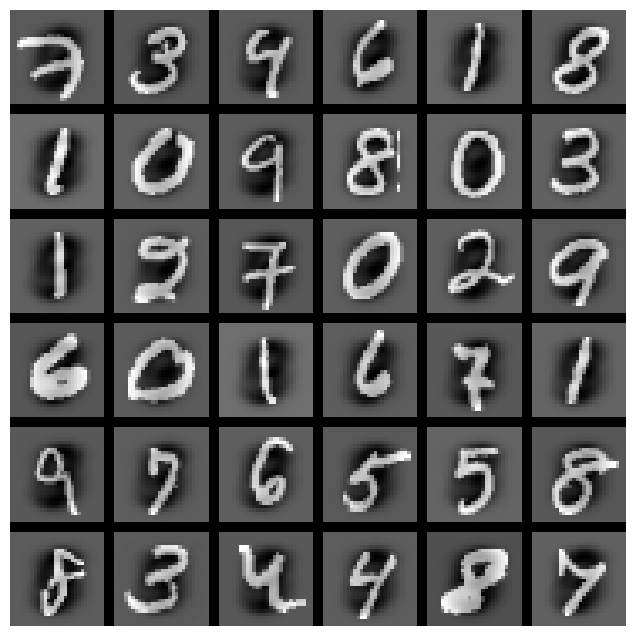
\includegraphics[width=0.6\textwidth]{image_02}
                \caption{MNIST Dataset}
            \end{figure}

    \pagebreak

            \subsubsection{Model Training with Fixed Learning Rate}
                Use the following code to train a neural network with fixed learning rate.
                \begin{codeblock}{Model Training with Fixed Learning Rate}
                    input_size = 28 * 28 * 1
                    hidden_size = 50
                    num_classes = 10
                    net = TwoLayerNet(input_size, hidden_size, num_classes)

                    # Train the network
                    stats = net.train(
                        X_train,
                        y_train,
                        X_val,
                        y_val,
                        num_iters=2000,
                        batch_size=200,
                        learning_rate=1e-4,
                        learning_rate_decay=1,
                        reg=0,
                        verbose=True,
                    )

                    # Predict on the validation set
                    val_acc = (net.predict(X_val) == y_val).mean()
                    print("Validation accuracy: ", val_acc)
                \end{codeblock}

                The validation accuracy of model with fixed learning rate is equal to 0.8922.

    \pagebreak

            \subsubsection{Model Training with Decay Learning Rate}
                Use the following code to train a neural network with decay learning rate.
                \begin{codeblock}{Model Training with Fixed Learning Rate}
                    net = TwoLayerNet(input_size, hidden_size, num_classes)
                    stats_LRDecay = net.train(
                        X_train,
                        y_train,
                        X_val,
                        y_val,
                        num_iters=2000,
                        batch_size=200,
                        learning_rate=5e-4,
                        learning_rate_decay=0.95,
                        reg=0,
                        verbose=True,
                    )

                    # Predict on the validation set
                    val_acc_LRDecay = (net.predict(X_val) == y_val).mean()
                    print("Validation accuracy: ", val_acc_LRDecay)
                \end{codeblock}

                The validation accuracy of model with decay learning rate is equal to 0.9432.

    \pagebreak

            \subsubsection{Model Comparison}
                Now, we are plotting a graph to compare the loss of the model with fixed learning rate and the model with decay learning rate as shown below:
                \begin{figure}[h]
                    \centering
                    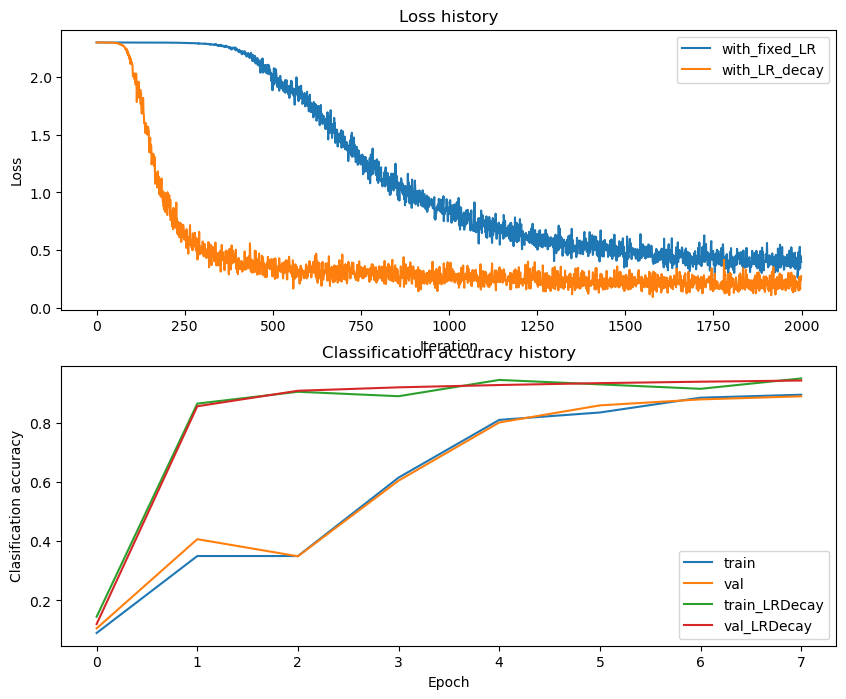
\includegraphics[width=\textwidth]{image_03}
                    \caption{Loss Comparison}
                \end{figure}
    
    \pagebreak

            \subsubsection{Weights Visualization}
                To get more insight of the model, we can visualize the weights that were learned in the first layer of the neural network as shown below:
                \begin{figure}[h]
                    \centering
                    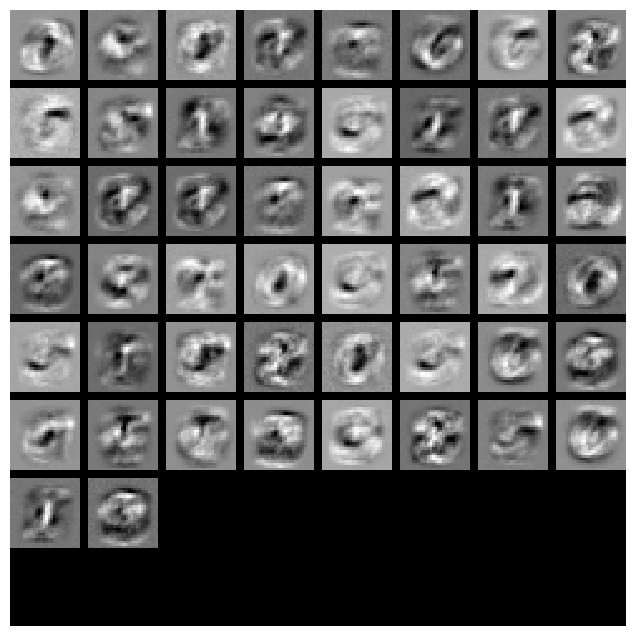
\includegraphics[width=0.6\textwidth]{image_04}
                    \caption{Weights Visualization}
                \end{figure}

    \pagebreak
        \subsection{Problem T12}
            \subsubsection{Implementation}
                Tuning the hyper-parameters and developing intuition for how they affect the final performance is a large part of using neural networks, so we want you to get a lot of practice.
                Below, you should experiment with different values of the various hyper-parameters, including hidden layer size, learning rate, number of training epochs, and regularization strength.
                You might also consider tuning the learning rate decay, but you should be able to get good performance using the default value.
                
                You should be aim to achieve a classification accuracy of greater than 97.4\% on the validation set.

                Your goal in this exercise is to get as good of a result on MNIST as you can, with a fully-connected neural network.
                Feel free implement your own techniques (e.g. PCA to reduce dimensionality, or adding dropout, or adding features to the solver, etc.).

                \vspace{1em}

                In this section, we will using grid search technique to find the best hyper-parameters.

                \vspace{1em}

                First, initialize the variables to store the best model and the best validation accuracy value for comparison.
                \begin{codeblock}{Initialize Variables}
                    best_net = None
                    best_val = -1
                \end{codeblock}

                Then, define the hyperparameter we want to perform grid search technique on.
                \begin{codeblock}{Define Hyperparameter}
                    HIDDEN_SIZE = [128, 256]
                    LEARNING_RATES = [1e-3, 2e-3]
                    REGULARIZATION_STRENGTHS = [0.0, 0.01, 0.1]
                    NUMBER_OF_ITERATIONS = 3000
                \end{codeblock}

                The next step is in the next page $\rightarrow$

        \pagebreak

                Finally, preform grid search on all hyperparameter combinations possible.
                \begin{codeblock}{Grid Search}
                    for hs in HIDDEN_SIZE:
                        for lr in LEARNING_RATES:
                            for reg in REGULARIZATION_STRENGTHS:
                                # Initialize a new neural network
                                net = TwoLayerNet(input_size, hs, num_classes)

                                # Train the network
                                stats = net.train(
                                    X_train,
                                    y_train,
                                    X_val,
                                    y_val,
                                    num_iters=NUMBER_OF_ITERATIONS,
                                    batch_size=256,
                                    learning_rate=lr,
                                    learning_rate_decay=0.95,
                                    reg=reg,
                                    verbose=False,
                                )

                                # Predict on validation set
                                val_acc = (net.predict(X_val) == y_val).mean()
                                print(
                                    "hidden_size: %d, lr: %e, reg: %e, val accuracy: %f"
                                    % (hs, lr, reg, val_acc)
                                )

                                # Save if this is the best network seen so far
                                if val_acc > best_val:
                                    best_val = val_acc
                                    best_net = net

                    print("Best validation accuracy achieved: %f" % best_val)
                \end{codeblock}

            \subsubsection{Result}
                \begin{table}[h]
                    \centering
                    \begin{tabular}{|c|c|}
                        \hline
                        Metrics & Value \\
                        \hline \hline
                        Validation Accuracy & 98.04\% \\
                        Test Accuracy & 97.51\% \\
                        \hline
                    \end{tabular}
                    \caption{Model Evaluation}
                \end{table}

\end{document}
